\documentclass[conference]{IEEEtran}
\IEEEoverridecommandlockouts

\usepackage{cite}
\usepackage{amsmath}
\usepackage{amssymb}
\usepackage{graphicx}
\usepackage{url}
\renewcommand{\IEEEkeywordsname}{Keywords}
\graphicspath{{./}}

\begin{document}

\title{\textbf{The Energy Cost of Privacy in Federated Learning}}

\author{%
\IEEEauthorblockN{Imad Mahaya}
\IEEEauthorblockA{\textit{LaSTIC Laboratory} \\
\textit{University of Batna 2} \\
Batna, Algeria \\
imad.mahaya@univ-batna2.dz}
\and
\IEEEauthorblockN{Ali Behloul}
\IEEEauthorblockA{\textit{LaSTIC Laboratory} \\
\textit{University of Batna 2} \\
Batna, Algeria \\
a.behloul@univ-batna2.dz}
\and
\IEEEauthorblockN{Khaled Hamouid}
\IEEEauthorblockA{\textit{LaSTIC Laboratory} \\
\textit{University of Batna 2} \\
Batna, Algeria \\
k.hamouid@univ-batna2.dz}
}

\maketitle

% Raises IEEEtran's "et al." threshold to six names; see refs.bib.
\bstctlcite{BSTcontrol}

\begin{abstract}
Differential privacy in federated learning is evaluated along two axes,
privacy and utility. On battery-powered edge devices a third decides whether a
configuration is deployable at all, and it is not reported. We measure the
energy cost of example-level differential privacy applied locally at each
client, with NVML hardware counters differenced around each federated round,
sweeping the privacy budget on UCI-HAR, whose clients are the individual study
participants, and on CIFAR-10.
The cost separates in two. A fixed per-round overhead from per-sample
gradients and clipping costs $+51\%$ on HAR and $+34\%$ on CIFAR-10, with no
dependence on $\varepsilon$ that a permutation test over seeds resolves
($p = 0.27$ and $p = 0.79$); everything budget-dependent acts through the
number of rounds required, and is the larger term. Measured as
energy-to-target-accuracy, privacy is free at $0.40$ accuracy on HAR for $\varepsilon \geq 1$,
$5.7\times$ at $0.70$, and unbounded at $0.85$, which no budget we tested
reaches at any expenditure. Because the cost is paid in joules it inherits the
local carbon intensity: the premium attributable to privacy alone is
$106$--$148$~gCO$_2$eq per 1000 runs on Algeria's grid against $5.7$--$7.9$~g
in Norway, a quantity the privacy-utility framing cannot express. We also report a measurement hazard:
running the privacy accountant's noise calibration inside the timed loop
reproduced an entire apparent $\varepsilon$ trend.
\end{abstract}

\begin{IEEEkeywords}
federated learning, differential privacy, energy efficiency, green AI, carbon
footprint, edge computing, human activity recognition
\end{IEEEkeywords}

\section{Introduction}

Federated learning allows many devices to train a shared model without sending
their raw data anywhere. That property is often described as privacy
preserving, but on its own it is not. Model updates leak information about the
data that produced them, and gradients alone are enough to recover training
examples. Differential privacy closes this gap with a formal guarantee, and it
has become the standard defense~\cite{abadi2016deep, geyer2017differentially}.

The guarantee is not free. Its cost is measured in accuracy, and the
privacy-utility trade-off is now well mapped: a budget $\varepsilon$ is chosen, 
the resulting accuracy is reported, and the trade-off between them is 
the result~\cite{abadi2016deep, yousefpour2021opacus}. What is not reported is what the choice costs to run.
 
This matters because federated learning exists to serve battery-powered
devices. A privacy configuration a phone cannot afford to execute is not a
worse point on the privacy-utility curve; it is not on the curve at all.
Green AI established energy and carbon as quantities worth
measuring~\cite{schwartz2020green, strubell2019energy}, but attention has gone to large
centralized training, where one operator owns the hardware and can move the
job to a cleaner grid. Federated learning inverts both conditions.

Previous work approaches this and stops short. Wireless resource-allocation
studies minimize device energy under a privacy constraint~\cite{liu2020privacy, zhang2023communication,
mao2026providing, chen2023energy, ding2026energy}, but the energy there is an objective inside a convergence limit
rather than something measured and $\varepsilon$ is fixed by the problem
statement rather than varied. Convergence theory under client-level privacy
proves that an optimal number of aggregations exists and that training past it
degrades the model~\cite{wei2020federated, wei2021user, zhou2023optimizing}. Those results say where to
stop; they do not say what continuing costs, because a round is an abstract
unit in them. Close to us, Schwermer et al.~\cite{schwermer2023energy} instrumented a
physical edge testbed and reported energy with differential privacy enabled
against disabled in a single privacy setting.
 
What none of them produces is the shape of the cost across the budget. A
designer choosing $\varepsilon$ needs to know whether halving it doubles the
energy bill or puts the accuracy target completely out of reach, and those are
different decisions.
 
We measure that shape. Energy comes from NVML~\cite{corporation2024nvidia} (NVIDIA Management Library) 
hardware counters for each federated round, not from device power ratings, and the privacy
budget is accounted over the whole run rather than per round. The guarantee is
example-level, applied locally at each client so that it holds against an
untrusted server, with the budget held per client over the whole run. Our
primary dataset is UCI-HAR~\cite{anguita2013public}, where the federation's
clients are the individual volunteers who contributed the data, so the client
boundary is a real person rather than a synthetic partition. CIFAR-10 checks the same
effects on a harder benchmark.

The paper makes four claims. The cost of privacy separates into a fixed
per-round overhead from per-sample gradients and clipping and a convergence
penalty that acts through the round count; the two are different sizes and
call for different remedies. Measured against the accuracy a deployment
actually needs, the cost is not a multiplier but a ceiling above which no
expenditure buys the target. Under a tight budget, training past a certain
round spends energy and loses accuracy at the same time, so the stopping point
is set by the privacy budget, rather than by the task. Because the cost is
paid in joules, the premium attributable to privacy is a geographic quantity,
which the privacy-utility framing cannot express.
 
One further result concerns the measurement itself. Deriving the noise
multiplier requires a search over the privacy accountant, and that search
costs more for a loose budget than a tight one. Running inside the federated loop,
where the natural implementation places it, its cost arrives inside the
measurement window and scales with $\varepsilon$, taking the shape of a privacy cost. 
In one of our sweeps it produced the entire observed trend, and
nothing in the resulting numbers announced the problem. Any energy study of a
privacy mechanism is exposed to this, so we describe it and the controls that
remove it.
% Section II -- Related Work.
% Positioning: prior work either optimises energy under a DP constraint
% analytically, or measures one privacy setting. Neither sweeps epsilon with
% hardware counters, and none reports energy-to-target-accuracy.

\section{Related Work}

\subsection{Measuring the energy of training}

Green AI made energy and carbon reportable quantities rather than
externalities~\cite{schwartz2020green, strubell2019energy}, and a family of tools now estimates
them from utilization traces and grid factors~\cite{henderson2020towards, anthony2020carbontracker,
lacoste2019quantifying}. Comparisons of those tools against instrumented hardware find the
estimates diverge substantially from measurement~\cite{bouza2023estimate,
aquino2025towards}, which is why we read NVML counters rather than model power
from device ratings. Patterson et al.~\cite{patterson2021carbon} established that
where a job runs changes its emissions by $5$--$10\times$; we apply that to
the premium a privacy budget adds.

\subsection{Energy and differential privacy in federated learning}

One line of work treats DP noise as a constraint inside a wireless
resource-allocation problem and minimizes device energy under it, either by
harvesting channel noise as the privacy mechanism~\cite{liu2020privacy, zhang2023communication, mao2026providing} or by co-designing compression with the noise budget~\cite{chen2023energy, ding2026energy}. 
Energy there is an optimization objective evaluated
through a convergence bound; it is not measured and $\varepsilon$ is a
constraint rather than a swept variable. Closest to us empirically,
Schwermer et al.~\cite{schwermer2023energy} built a physically distributed edge testbed
and reported traffic, energy and training time for a CNN on MNIST with
differential privacy enabled, and found software estimates deviating by up to
$35\%$ from measurement. Their contrast is DP on versus off at one setting;
ours is the shape of the cost across the budget. Aroussi
et al.~\cite{aroussi2026adaptive} schedule $\varepsilon$ adaptively on Raspberry Pi and
ESP32 nodes and report a $20$--$25\%$ energy improvement over a fixed-privacy
baseline, the gain of a controller, rather than the cost curve. A designer
would need to choose the budget in the first place.

\subsection{Rounds as the mechanism}

That the cost should act through the round count is known analytically. Wei
et al.~\cite{wei2020federated} prove that under client-level DP there is an optimal
number of aggregations for a given protection level, beyond which
convergence degrades, and later derive a discounting method to find
it~\cite{wei2021user}; the same optimum reappears for personalized
FL~\cite{wei2023personalized}, for query and reply counts~\cite{zhou2023optimizing}, and in control
formulations that adapt noise and rounds jointly~\cite{yuan2025optimal}. These results
say where to stop. What they do not say is what continuing costs, because
the round is an abstract unit in them. Our measurements price it: on CIFAR-10 at $\varepsilon = 0.5$ the peak this
literature predicts falls at round 8 of 30, and the rounds after it are
priced in joules below.

\subsection{Our position}

We therefore contribute the missing empirical axis: hardware-counter energy
swept across $\varepsilon$ under whole-run per-client
accounting~\cite{abadi2016deep}, decomposed into a per-round overhead and a
convergence penalty, and reported as energy-to-target-accuracy rather than
energy per round or energy per run. Our guarantee is example-level and local,
weaker than the client-level protection of~\cite{geyer2017differentially,
wei2020federated}; the energy question is orthogonal to that choice, and the
per-round overhead we measure is the cost of the per-sample gradients that
both require.
\section{Methodology}

\subsection{Federated Setup}

Both datasets run on Flower~\cite{beutel2020flower} with FedAvg, $50\%$ of clients
sampled per round for training and $50\%$ for evaluation, one local epoch,
batch 32, SGD at lr $0.01$ with momentum $0.9$, three seeds per
configuration, and $\varepsilon \in \{0.5, 1, 2, 4, 8, \infty\}$ at
$\delta = 10^{-5}$. Neither model uses batch normalization, which
Opacus~\cite{yousefpour2021opacus} rejects because it mixes information across examples.

\textbf{UCI-HAR}~\cite{anguita2013public} is primary. We keep the published
subject-disjoint split: its 21 training participants become the federation's
clients, one per person, and the 9 test participants are held out, so central
accuracy measures generalization to people the federation never saw. The
partition is given by who contributed the data rather than by a heterogeneity
parameter. We train on the raw inertial signals (nine channels, 128 samples
per window) with a three-block 1D CNN and global average pooling ($37$k
parameters) for 100 rounds. Local train and validation sets are split
within each activity class, in file order, discarding the straddling window:
windows overlap by $50\%$, so a random split would leak, and the activities
come in blocks, so one ordered cut would drop classes.

\textbf{CIFAR-10} is secondary: a five-layer CNN ($62$k parameters) across 20
clients over 30 rounds, partitioned by a Dirichlet distribution over labels at
$\alpha = 0.5$~\cite{hsu2019measuring}.

The HAR round budget comes from the non-private convergence curve rather than
from convenience. Under whole-run accounting the number of rounds enters the
privacy calculation directly, so it is not a free parameter.

\subsection{Privacy Accounting}

We enforce \emph{example-level} differential privacy, applied locally:
Opacus~\cite{yousefpour2021opacus} clips and noises per-sample gradients
inside local training, so the guarantee protects one of a client's own
examples, the noise is added before anything leaves the device, so it holds
against an untrusted server, and each client holds its own $(\varepsilon,
\delta)$ budget over the whole run. This is weaker than the client-level
guarantee of~\cite{geyer2017differentially, wei2020federated}, which noises
the entire client update and conceals participation itself; the per-round
overhead we measure is the per-sample gradient work both need. The budget is
accounted over every local SGD step across every round a client joins, not per
round and not per epoch. For a client with $n$ examples, batch $B$, $R$
rounds, sampling fraction $q_c$ and $E$ local epochs:
%
\begin{equation}\label{eq:steps}
  s_{\text{total}} = R \, q_c \, E \, \lceil n / B \rceil
\end{equation}
%
We invert the RDP accountant~\cite{mironov2017renyi} once, before training, to obtain the
noise multiplier $\sigma$ giving the target $\varepsilon$ after
$s_{\text{total}}$ steps, and hold it constant. Precomputing is deliberate: in
simulation each client is reconstructed every round, so an engine-internal
accountant resets each round and reports a per-round $\varepsilon$ while the
true budget compounds. Opacus samples at a rate $1/\lceil n/B \rceil$ rather
than $B/n$, and we calibrate at the rate the sampler uses. We claim no
amplification by client subsampling, which would require secure aggregation or
a shuffler.

The $q_c$ in \eqref{eq:steps} makes $s_{\text{total}}$ an \emph{expected}
participation count, and nothing in the protocol bounds the realised one,
which is binomial. So $\sigma$ is calibrated optimistically: recomputing each
client's spent $\varepsilon$ from the participation log, the worst client
overspends in every private run we measured, by $4$--$22\%$
(Table~\ref{tab:perround}, last column). A guarantee that must hold
unconditionally has to drop $q_c$ and calibrate against $R \, E \, \lceil n/B
\rceil$, or cap participation per client; we report the target
$\varepsilon$ as the design parameter it is, with the realised worst case
beside it.

Because per-client dataset sizes differ, $\sigma$ differs per client, and the
two datasets sit in different regimes: a HAR client holds far fewer examples,
which raises the sampling rate, and runs a longer schedule. Both push $\sigma$ up.

\subsection{Energy Measurement}

Energy comes from the NVML counter, which accumulates
millijoules on the device. Differencing it around each round requires no power
sampling and no integration and cannot miss a transient. Measurement is
server-side; all clients
share one GPU in simulation, so a round-level window captures the full cost
regardless of actor scheduling, whereas measuring inside each client would
double-count concurrent work.

Every energy figure in this paper is net of the idle baseline unless a column
is labelled Gross. We report both, the baseline sampled per run after board
power settles, since a card does not reach its floor the moment a run
ends and probing during that tail reads a busy baseline. Baselines are checked
against the sweep median, and outliers are discarded. Net energy subtracts the
baseline over the wall clock the counter covers, excluding start-up, central
evaluation and teardown. The three seeds also give measurement noise floors, each the worst
within-condition spread across seeds and each measured on the quantity it
bounds --- energy per round, board power, final accuracy --- and reported in
Section~\ref{sec:Results}; no smaller difference is treated as an effect.
Where a claim is about an ordering across budgets rather than a single
difference, a floor is the wrong instrument, because the quantity on trial is
the spread of the condition means: there we permute the seed labels across
the five private budgets and report the $p$-value of the resulting $F$.

\subsection{Experimental Controls}
\label{sec:controls}

We fix the clipping norm $C = 1.0$ for all $\varepsilon$ values to isolate 
the effect of privacy. We verify each round that the number of optimizer steps 
matches the privacy accountant's calibration. All noise scales $\sigma$
 are computed before timing, since the accountant's search time varies with 
$\varepsilon$ and could otherwise create a false energy trend. We randomize the order of 
$\varepsilon$ values to separate privacy effects from execution-order drift. 
We do not force deterministic GPU kernels, as this can change kernel selection and energy use. 
Instead, we assess reproducibility across multiple random seeds.

\subsection{Limitations}

Clients are virtual and share one GPU, although on HAR each holds one real
participant's data. CPU RAPL counters were unavailable, so measurement is
GPU-only and communication energy is modeled. The workload does not saturate
the device, which is why net figures accompany gross ones. Per-channel
standardization constants come from the training split and are global across
clients, so a real deployment would have to agree them without pooling raw
data. And the HAR round budget is set from the non-private convergence curve,
so private conditions inherit a longer schedule than any of them needs and a
larger $\sigma$ with it; their accuracies are a lower bound on what a
per-$\varepsilon$ tuned budget would give.

% Figure environments. All three are the UCI-HAR sweep, to match Section IV.
% Regenerate with `python analyze.py results_har/`, which writes the PNGs into
% results_har/; copy them beside main.tex (graphicspath is ./ only, on purpose
% -- results/ holds identically named CIFAR-10 figures).
% Inputted before Section IV in main.tex: floats only move forward.

\begin{figure}[t]
\centering
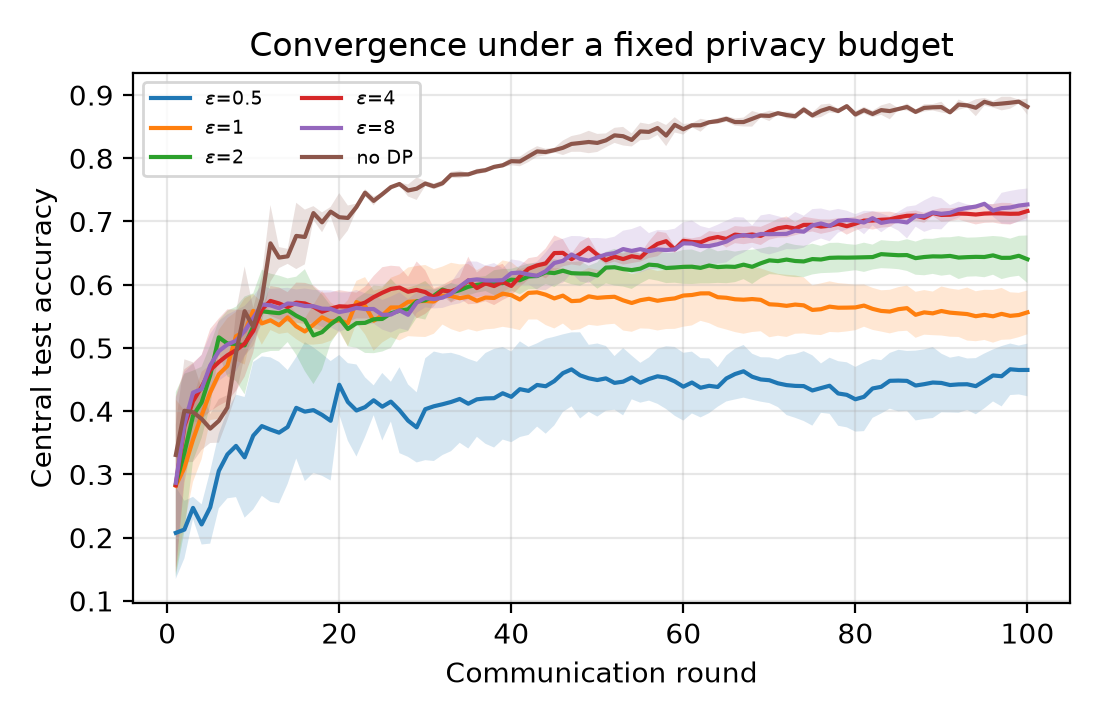
\includegraphics[width=\columnwidth]{fig1_convergence.png}
\caption{Central test accuracy per round on UCI-HAR, mean $\pm 1$ SD over
three seeds. No stopping round is marked: on HAR no peak-to-final drop clears
the across-seed spread.}
\label{fig:convergence}
\end{figure}

% fig2 (energy to target) dropped: Table~\ref{tab:target} carries the same
% numbers with the unreached cells legible, which a bar chart cannot show.

% \begin{figure}[t]
% \centering
% 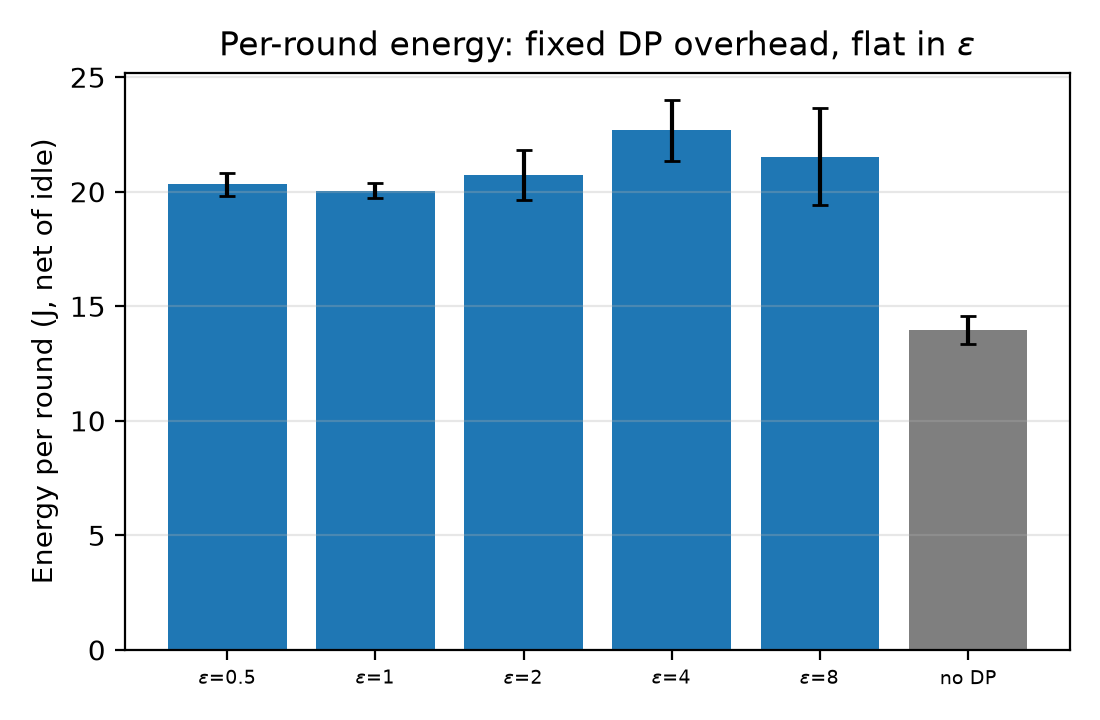
\includegraphics[width=\columnwidth]{fig3_energy_per_round.png}
% \caption{Energy per round on UCI-HAR by privacy budget, net of idle, with the
% non-private baseline in grey and $\pm 1$ SD over three seeds. Private training
% costs $21.1$~J per round against $14.0$~J, an overhead of $+51\%$, The spread across the five private conditions is $12.5\%$ of that mean against a $7.8\%$ noise floor, so we claim no systematic dependence on $\varepsilon$ rather than equality. This separates the two mechanisms: the step
% is an implementation overhead independent of $\varepsilon$, so every
% budget-dependent cost acts through the round count.}
% \label{fig:perround}
% \end{figure}

\begin{figure}[t]
\centering
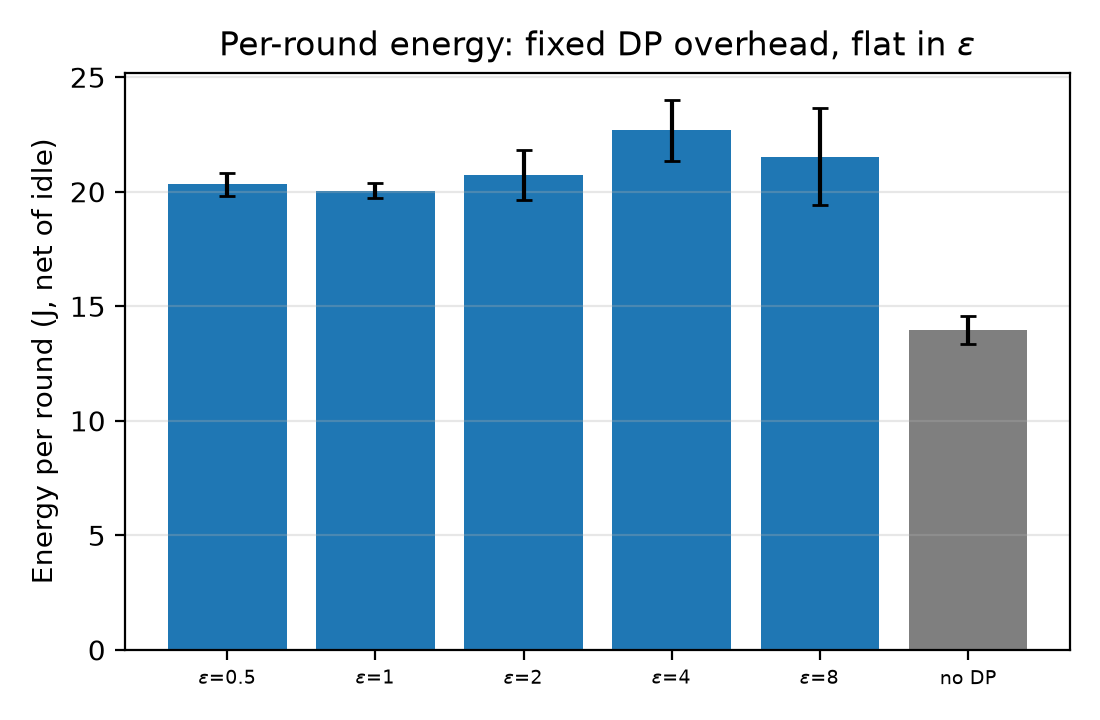
\includegraphics[width=\columnwidth]{fig3_energy_per_round.png}
\caption{Net energy per round on UCI-HAR, mean $\pm 1$ SD over three seeds;
non-private baseline in grey.}
\label{fig:perround}
\end{figure}


% fig4 (carbon by grid) dropped: Table~\ref{tab:carbon} is the same six
% numbers, and the reviewers asked for the redundancy to go first.


% Section IV -- Results.
% PROVENANCE. Every number below is printed by analyze.py from the run JSONs
% committed in this repository. Regenerate, do not retype:
%   HAR     : analyze.py results_har/ --latex --targets 0.40,0.50,0.70,0.85
%             --sigma-from results/ --realised-eps spent_har.json
%   CIFAR-10: analyze.py results/ --latex --targets 0.15,0.20,0.25
%             --realised-eps spent_cifar.json
%   ablations: analyze.py results_ablation_har/ --ablation ; same on results_ablation/
%   stopping : per_seed_peak.py results_har/ ; per_seed_peak.py results/

\section{Results}

Every figure is a mean over three seeds. Two resolutions bound what we claim:
the energy floor, the worst within-condition across-seed spread of board
power, is $\pm 4.89$~W ($7.80\%$) on HAR and $\pm 5.94$~W ($8.91\%$) on
CIFAR-10; the accuracy floor, the same statistic on final accuracy, is
$\pm 0.051$ on HAR and $\pm 0.031$ on CIFAR-10. No smaller difference is
reported as an effect.

The HAR sweep passes every gate: $18/18$ runs, wall-clock flat to $0.3\%$
across the private conditions against $38.0$~s without privacy, and 89
optimiser steps per round throughout. On CIFAR-10 one $\varepsilon = 4$ run
was measured a month after the others and is excluded for breaking the
flatness gate; including it moves the mean overhead from $+34\%$ to $+36\%$,
inside the floor either way, so that condition is reported on two seeds.

\subsection{The Per-Round Cost Is Power Times Time}

Net of idle, private training costs $21.1$~J per round on HAR against
$14.0$~J, and $107.9$~J against $80.4$~J on CIFAR-10 --- $+51\%$ and $+34\%$
(Table~\ref{tab:perround}). Two numbers that far apart look like an unstable
measurement until they are decomposed. Private rounds draw more power
\emph{and} last longer, and the two factors behave differently:

\begin{center}
\begin{tabular}{lrrr}
\hline
 & Power & Duration & Energy \\
\hline
UCI-HAR  & $1.190\times$ & $1.267\times$ & $1.507\times$ \\
CIFAR-10 & $1.196\times$ & $1.132\times$ & $1.354\times$ \\
\hline
\end{tabular}
\end{center}

The power factor is the same to within $0.5\%$ across two datasets with
different models, different input shapes and a $4\times$ difference in model
size: the arithmetic of per-sample gradients and clipping, apparently a
hardware constant. The time factor is not, depending on how the workload fills
the device.

Neither orders with $\varepsilon$. The overhead runs $+45.4\%$, $+43.4\%$,
$+48.3\%$, $+62.2\%$, $+54.0\%$ on HAR and $+36.0\%$, $+38.6\%$, $+30.7\%$,
$+30.6\%$, $+35.6\%$ on CIFAR-10, non-monotone in both. On CIFAR-10 the spread
across budgets is $6.0\%$ of the mean, inside the $8.91\%$ floor, so the
per-round cost is $\varepsilon$-independent within resolution; on HAR it is
$12.5\%$ against $7.80\%$, not resolvably flat, but being non-monotone it is
scatter above our resolution rather than a budget effect. Either way the
per-round cost carries no systematic budget dependence, which is what the rest
of this section rests on.

\subsection{The Cost Grows with the Accuracy Demanded}

Measured against the quality a deployment wants, the cost is not flat at all
(Table~\ref{tab:target}, Fig.~\ref{fig:convergence}). On HAR, reaching $0.40$
accuracy costs $185$--$357$~J
net whether or not privacy is on: at this quality privacy is free. At $0.50$
the private conditions cost $1.28$--$1.79\times$ the non-private $197$~J. At
$0.70$ only $\varepsilon \ge 4$ arrives at all, at $1710$~J against $301$~J, a
factor of $\mathbf{5.7}$. At $0.85$, which the non-private model reaches in
$57.0$ rounds and $839$~J, no budget we tested arrives at any expenditure.

CIFAR-10 shows the same shape at its own scale: $0.15$ costs $644$--$760$~J
against $611$~J, $0.20$ costs $1.40$--$1.63\times$ the non-private $677$~J,
and $0.25$ is reached only at $\varepsilon \ge 2$, at $1.96$--$2.29\times$.

Unreachability is the sharpest form of the cost: above a budget-dependent
ceiling the accuracy cannot be bought at all, because the extra training that
would close the gap is itself what raises $\sigma$.

\subsection{A Stopping Round Appears Only Under a Tight Budget}

Under a tight enough budget the accuracy curve peaks and declines, so training
past the peak spends energy and loses accuracy at once. Whether a peak is
resolvable is a question about noise rather than about the argmax, so we mark
a stopping round only where the peak-to-final drop exceeds the across-seed
spread of final accuracy in that condition.

Two CIFAR-10 budgets qualify (Fig.~\ref{fig:stopping}). At
$\varepsilon = 0.5$ the mean curve peaks at $0.176$ at round 8 and ends at
$0.150$ --- a drop of $0.026$ against a $\pm 0.010$ spread, the three seeds
peaking at rounds 8, 8 and 9 --- and the rounds after the peak account for
$60$--$68\%$ of the run's net energy. At $\varepsilon = 1$ the drop is $0.044$
against $\pm 0.014$, the seeds peak between rounds 10 and 16, and
$42$--$61\%$ of the energy falls after it. At $\varepsilon \ge 2$, and without
privacy, no decline clears the spread within 30 rounds.

UCI-HAR produces no resolvable stopping round at any budget: its largest drop
is $0.032$ at $\varepsilon = 1$ against a $\pm 0.042$ spread, and at
$\varepsilon = 0.5$ its seeds peak at rounds 16, 54 and 65 while the mean
curve peaks at round 98 --- an argmax wandering over a plateau, not a decline.
With $\sigma$ near $20$ the model never climbs far enough to have anything to
give back. The effect is therefore real but conditional, with the threshold
between $\varepsilon = 1$ and $\varepsilon = 2$ on CIFAR-10.

\subsection{Under a Tight Budget, Tuning Stops Working --- On One Task}

We vary one factor at a time at $\varepsilon \in \{1, \infty\}$ with three
seeds per cell, reading every difference against floors measured within a
cell: $\pm 0.041$ on accuracy for HAR, $\pm 0.024$ for CIFAR-10.

\textbf{On HAR the private model is noise-limited.} At $\varepsilon = 1$ final
accuracy spans $0.037$ across one, two and five local epochs and $0.018$
across $C \in \{0.5, 1, 2\}$, both inside the floor and both non-monotone.
\textbf{On CIFAR-10 the same two knobs are decisive}, falling monotonically
from $0.182$ to $0.114$ to $0.100$ across the epoch axis ($3.4\times$ the
floor) and from $0.213$ to $0.182$ to $0.100$ across the clipping axis
($4.7\times$). The identical experiment is inert on one task and dominant on
the other, and the floors say why: CIFAR-10 resolves accuracy twice as finely
while its private model retains more signal to lose.

\textbf{The standard efficiency lever stops paying.} More local work per round
is how federated learning ordinarily buys fewer rounds, and without privacy it
works: on HAR the energy to reach $0.70$ falls from $345$~J at one local epoch
to $193$~J at five. Under $\varepsilon = 1$ the target is reached at no epoch
count while energy per round rises from $22$~J to $49$~J, and on CIFAR-10 it
is worse than useless --- accuracy collapses while post-peak waste grows from
$1785$~J to $7312$~J. Local steps enter $s_{\text{total}}$, so extra local
work forces a larger $\sigma$ and cancels the convergence gain it bought.

\textbf{Clipping is free in compute.} $C$ leaves energy per round unchanged
($22$~J at all three values on HAR, $112$--$119$~J on CIFAR-10), so it acts
purely through convergence, in a way final accuracy alone hides: $C = 2$ peaks
at $0.187$ at round 7 and ends at $0.100$, giving back $46.7\%$ of its peak
against $2.7\%$ at $C = 0.5$. Our fixed $C = 1.0$ is conservative rather than
optimal.

\subsection{Carbon Cost by Grid}

Table~\ref{tab:carbon} scales the measured HAR energy
to 1000 runs and apply published grid carbon intensities, repeating the
measured workload rather than extrapolating to other hardware. The cost
attributable to privacy runs from $106$--$148$~gCO$_2$eq on Algeria's
gas-dominated grid to $5.7$--$7.9$~g in Norway, a factor of $18.8$ for the
same computation and the same guarantee. CIFAR-10 gives $115$--$146$~g against
$6.1$--$7.8$~g, the same premium despite a workload five times larger per
round. Selecting a privacy budget is therefore partly a geographic decision,
which the privacy--utility framing cannot express.

\begin{table}[t]
\caption{Energy to reach a target accuracy on UCI-HAR (J net of idle; rounds
in parentheses). ``---'' marks targets not reached within 100 rounds.
$\ddagger$: 2 of 3 seeds}
\label{tab:target}
\centering
\begin{tabular}{lrrrr}
\hline
$\varepsilon$ & 0.40 & 0.50 & 0.70 & 0.85 \\
\hline
0.5      & 357 (13.0) & 334$\ddagger$ (12.0) & --- & --- \\
1        & 201 (4.7) & 258 (7.7) & --- & --- \\
2        & 197 (4.0) & 353 (12.0) & --- & --- \\
4        & 210 (4.3) & 253 (6.3) & 1710 (74.3) & --- \\
8        & 187 (3.3) & 269 (7.7) & 1699 (76.3) & --- \\
$\infty$ & 185 (6.0) & 197 (7.0) & 301 (15.0) & 839 (57.0) \\
\hline
\end{tabular}
\end{table}

\begin{table}[t]
\caption{gCO$_2$eq per 1000 UCI-HAR training runs. ``Privacy'' is the private
minus non-private difference across $\varepsilon$}
\label{tab:carbon}
\centering
\begin{tabular}{lrrr}
\hline
Grid & DP & No DP & Privacy \\
\hline
Norway  &  21 &  15 &    6--8 \\
France  &  46 &  32 &  12--17 \\
Algeria & 403 & 281 & 106--148 \\
India   & 521 & 363 & 137--191 \\
\hline
\end{tabular}
\end{table}

% Section V -- Discussion (second cut, for the six-page limit). Every number
% appears in Section IV. Nothing here restates a number the conclusion needs.

\section{Discussion}

% \subsection{Two Costs, Two Remedies}

% The fixed per-round cost comes from DP operations and can be reduced through implementation improvements. The larger convergence cost comes from the extra rounds required by the privacy budget and must be addressed through the round budget. Per-round energy captures only the first cost, while energy-to-accuracy reveals the larger cost. Thus, energy measurement helps determine where optimization effort should focus.

\subsection{Privacy Sets a Quality Ceiling}

Separating the two costs matters because they admit different remedies: the fixed overhead is an implementation problem, the convergence penalty a scheduling one, and per-round energy sees only the first.

Privacy does not impose a constant energy overhead: on HAR, it is negligible at $0.40$ accuracy, rises to $5.7\times$ at $0.70$, and becomes unbounded at $0.85$. Beyond this point, additional computation does not improve accuracy. Privacy and target utility should therefore be chosen jointly rather than sequentially.

The reason is that the round budget affects the privacy budget. More client participation requires more noise to maintain the same $\varepsilon$; on HAR, increasing rounds raises $\sigma$ and training longer can become counterproductive. A stopping rule is therefore needed, although its exact threshold depends on the dataset and privacy budget.

\subsection{When the Model Is Noise-Limited, Tuning Is Not the Lever}

Our HAR ablations are negative and useful. At $\varepsilon = 1$ neither local
epochs nor the clipping norm moves accuracy by more than $3\%$ against a
$7.8\%$ floor, so a practitioner responding to a disappointing private model
by sweeping hyperparameters will spend considerable energy to land where they
started. This does not hold in every regime, and CIFAR-10 shows why: there the
private model retains more signal, and the same settings can be got badly
wrong. Increasing local work per round is the standard way to reduce
communication in federated learning; under DP it stops paying on HAR and
actively harms on CIFAR-10, because local steps enter the budget and force a
larger $\sigma$.

\subsection{Where the Computation Runs}

% Measured in joules, the cost inherits the carbon intensity of wherever they
% are drawn: a $21.4\times$ range between Algeria's grid and Norway's for
% identical computation and an identical guarantee. The point is sharper for
% federated learning than for centralized training, because the computation
% sits on whatever grids the participating devices do, and no operator chooses
% them. A deployment cannot relocate the way a data center can; what it can
% adjust is how much computation the privacy requirement demands.
The geographic point is sharper for federated learning than for centralized training. The computation sits on whatever grids the participating devices do, and no operator chooses them. A deployment cannot relocate the way a data center can; what it can adjust is how much computation the privacy requirement demands.

\subsection{Measuring Energy Around a Privacy Accountant}

Instrumentation attached to a privacy mechanism tends to scale with the
privacy parameter, so its cost mimics the effect under study. The accountant's
noise-calibration search is the case we hit: running inside the federated loop, it
reproduced our entire observed $\varepsilon$ trend, while executed step counts
stayed flat, and nothing in the resulting numbers announces this. We recommend
three controls: derive noise multipliers before measurement begins, verify per
round that executed and calibrated step counts agree, and randomize run order
so that drift over a sweep cannot be mistaken for an $\varepsilon$ effect.

\subsection{Threats to Validity}

Clients are virtual and share one GPU, so the ratios transfer to real devices,
but the absolute joules do not; confirming them on physical hardware is the
immediate next step. Measurement is GPU-only and communication energy is
modelled --- for a $0.15$--$0.24$~MB model over tens of rounds we expect it
small, but have not shown it. Two datasets bound the effects rather than
establishing them. And our accounting claims no amplification by subsampling,
so the reported $\varepsilon$ is an upper bound: these are the costs under the
weakest trust assumptions, not the best achievable.

\section{Conclusion}

 We measured the energy cost of differential privacy in federated learning using hardware counters around each round on UCI-HAR and CIFAR-10.

 The cost has two components. A fixed per-round overhead from per-sample gradients and clipping adds $51\%$ on HAR and $34\%$ on CIFAR-10, in neither case ordered in $\varepsilon$. The larger cost comes from the additional rounds required to reach a target accuracy: reaching $0.70$ on HAR requires $5.7\times$ the non-private energy at $\varepsilon=4$, while $\varepsilon\le2$ does not reach the target.

 Three practical implications follow. First, set the round budget from the privacy budget rather than the task, since additional rounds consume privacy budget and can become counterproductive. At $\varepsilon=0.5$ on CIFAR-10, two thirds of the run's energy is spent after the accuracy peak. Second, choose the privacy budget and target accuracy jointly because privacy can impose an accuracy ceiling. Third, when the model is noise-limited, hyperparameter tuning provides little benefit.

 Finally, energy measurements can be biased by privacy-accounting overhead. We therefore recommend precomputing noise multipliers, verifying step counts, and randomizing run order. Future work should identify when the system shifts from implementation-limited to noise-limited behavior.


\bibliographystyle{IEEEtran}
\bibliography{refs}

\end{document}